Before comparing forecasters, we ask which properties of the RTT carry over from the 6\,s input window to the 3\,s horizon. The statistics use the measured pings of the training sessions, each centered on its own mean, with session-bootstrap confidence intervals (script \texttt{fr\_volatility.py}).

\begin{figure}[htbp]
  \centering
  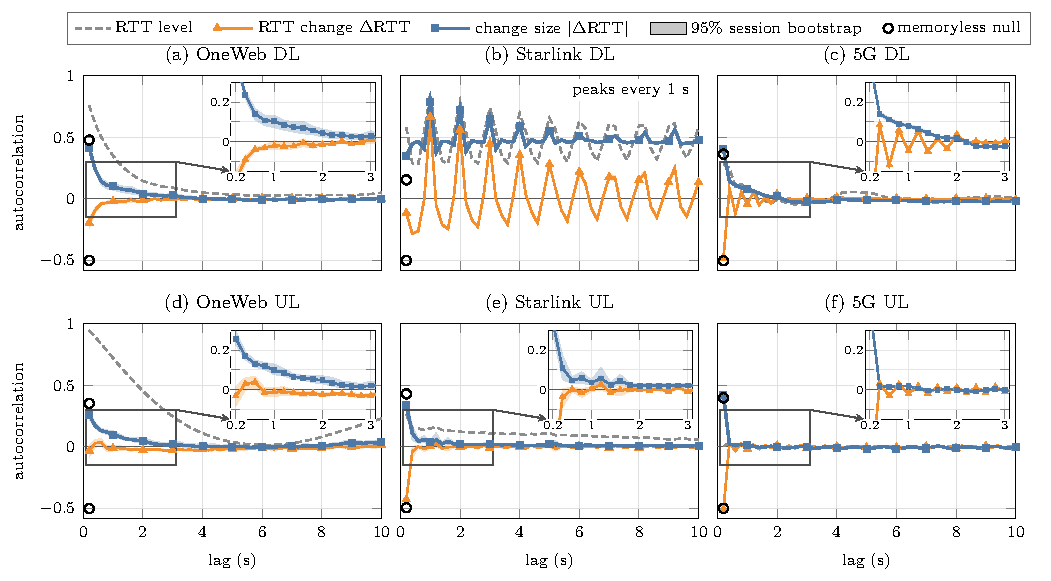
\includegraphics[width=\linewidth]{figs_pdf/fr_volatility.pdf}
  \caption{Autocorrelation of the RTT level, of its 200\,ms change $\Delta$RTT, and of the size of the change $|\Delta\mathrm{RTT}|$ in the training sessions (shaded: 95\% session-bootstrap interval). Circles: value of a memoryless series at 0.2\,s. Insets: lags of 0.2 to 3\,s. Starlink DL peaks every second because of a load-driven sawtooth.}
  \label{fig:vol}
\end{figure}

\paragraph{The next change is hard to predict, the level reverts.} From 0.4\,s to 10\,s the autocorrelation of $\Delta$RTT stays within $\pm$\VolDmaxAbs{} on five links (Fig.~\ref{fig:vol}). Past changes say almost nothing about the next change. The direction is still partly predictable because the RTT returns toward its recent level. Expecting a return to the mean of the input gets the sign of the 1\,s change right in \VolSignRevLo\% to \VolSignRevHi\% of the test windows (balanced accuracy), and the learned forecasters reach \VolSignNNLo\% to \VolSignNNHi\%. Point forecasts beat persistence mainly by not repeating the last, noisy ping. Their MAE is \PersRatioLo{} to \PersRatioHi{} times lower than that of persistence, but none of them gets much closer to the next value than the others, which is why the RMSE hardly separates them.

\paragraph{The spread depends on the link state.} On OneWeb and 5G, the SD of the 6\,s input does not predict the error of a 1\,s forecast within a session (rank correlation \VolWithinLo{} to \VolWithinHi), but it does between sessions (\VolBetweenLo{} to \VolBetweenHi). Each session runs in a noise regime set by its load and radio conditions, and a few seconds of input reveal it. Starlink DL is different. Under the saturating downlink test its RTT climbs from about 35\,ms to about 200\,ms in steps of about 50\,ms and drops back once per second. The sawtooth switches on and off within a session, and the volatility of the last 6\,s predicts that of the next 3\,s (within-session rank correlation \VolSLDLrv). We attribute it to queue build-up and drain under load, since the uplink test does not show it.

\paragraph{Errors are skewed upward.} Queues and retransmissions add delay, while nothing removes delay below the propagation floor. For the 1\,s forecasts of the initial model, the 97.5\% error quantile is \SkewQUL{} times the size of the 2.5\% quantile on 5G UL and \SkewOWDL{} times on OneWeb DL.

\paragraph{Consequence.} A constant-width interval around a point forecast, as in the previous report, ignores both properties. Calibrated to cover 95\% of all windows, it covers \CovConstCalmLo{} to \CovConstCalmHi{} of the calmest tenth and \CovConstVolLo{} to \CovConstVolHi{} of the most volatile tenth. Because the interval score is minimized by the conditional quantiles~\cite{gneiting2007strictly}, a forecaster should learn the spread and its skew from the input and be calibrated on sessions it has not seen. Fig.~\ref{fig:trace1min} shows the result on one minute of Starlink DL.

\begin{figure}[htbp]
  \centering
  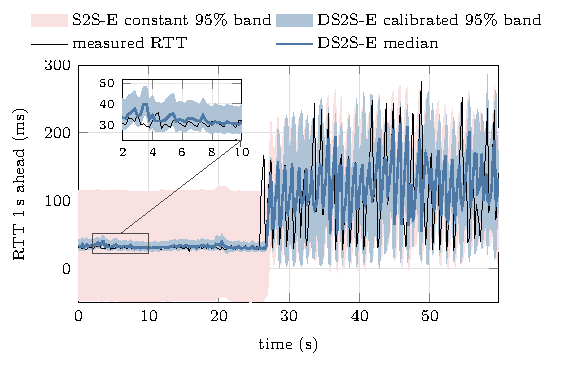
\includegraphics[width=0.95\linewidth]{figs_pdf/fr_trace.pdf}
  \caption{One minute of a Starlink DL test session, forecast 1\,s ahead. The initial model (S2S-E) has a constant 95\% interval of \TraceWidS\,ms. The calibrated interval of the final model (DS2S-E) is \TraceWidDCalm\,ms wide (median) while the link is quiet and \TraceWidDLoad\,ms once it swings. Inset: the quiet part.}
  \label{fig:trace1min}
\end{figure}
